\begin{figure}[H]
	\centering
	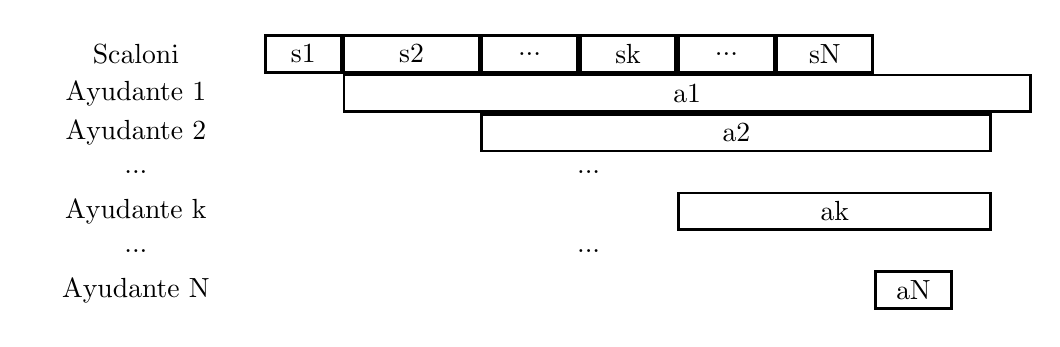
\begin{tikzpicture}
	% Paths, nodes and wires:
	\node[shape=rectangle, draw, line width=1pt, minimum width=0.965cm, minimum height=0.465cm] at (3.5, 5.75){} node[anchor=center, align=center, text width=0.577cm, inner sep=6pt] at (3.5, 5.75){s1};
	\node[shape=rectangle, draw, line width=1pt, minimum width=1.715cm, minimum height=0.465cm] at (4.875, 5.75){} node[anchor=center, align=center, text width=1.327cm, inner sep=6pt] at (4.875, 5.75){s2};
	\node[shape=rectangle, draw, line width=1pt, minimum width=8.715cm, minimum height=0.465cm] at (8.375, 5.25){} node[anchor=center, align=center, text width=8.327cm, inner sep=6pt] at (8.375, 5.25){a1};
	\node[shape=rectangle, draw, line width=1pt, minimum width=6.465cm, minimum height=0.465cm] at (9, 4.75){} node[anchor=center, align=center, text width=6.077cm, inner sep=6pt] at (9, 4.75){a2};
	\node[shape=rectangle, draw, line width=1pt, minimum width=1.215cm, minimum height=0.465cm] at (6.375, 5.75){} node[anchor=center, align=center, text width=0.827cm, inner sep=6pt] at (6.375, 5.75){...};
	\node[shape=rectangle, draw, line width=1pt, minimum width=1.215cm, minimum height=0.465cm] at (7.625, 5.75){} node[anchor=center, align=center, text width=0.827cm, inner sep=6pt] at (7.625, 5.75){sk};
	\node[shape=rectangle, draw, line width=1pt, minimum width=3.965cm, minimum height=0.465cm] at (10.25, 3.75){} node[anchor=center, align=center, text width=3.577cm, inner sep=6pt] at (10.25, 3.75){ak};
	\node[shape=rectangle, draw, line width=1pt, minimum width=1.215cm, minimum height=0.465cm] at (8.875, 5.75){} node[anchor=center, align=center, text width=0.827cm, inner sep=6pt] at (8.875, 5.75){...};
	\node[shape=rectangle, draw, line width=1pt, minimum width=1.215cm, minimum height=0.465cm] at (10.125, 5.75){} node[anchor=center, align=center, text width=0.827cm, inner sep=6pt] at (10.125, 5.75){sN};
	\node[shape=rectangle, draw, line width=1pt, minimum width=0.965cm, minimum height=0.465cm] at (11.25, 2.75){} node[anchor=center, align=center, text width=0.577cm, inner sep=6pt] at (11.25, 2.75){aN};
	\node[shape=rectangle, minimum width=2.715cm, minimum height=0.465cm] at (1.375, 5.75){} node[anchor=center, align=center, text width=2.327cm, inner sep=6pt] at (1.375, 5.75){Scaloni};
	\node[shape=rectangle, minimum width=2.715cm, minimum height=0.465cm] at (1.375, 5.25){} node[anchor=center, align=center, text width=2.327cm, inner sep=6pt] at (1.375, 5.25){Ayudante 1};
	\node[shape=rectangle, minimum width=2.715cm, minimum height=0.465cm] at (1.375, 4.75){} node[anchor=center, align=center, text width=2.327cm, inner sep=6pt] at (1.375, 4.75){Ayudante 2};
	\node[shape=rectangle, minimum width=2.715cm, minimum height=0.465cm] at (1.375, 3.75){} node[anchor=center, align=center, text width=2.327cm, inner sep=6pt] at (1.375, 3.75){Ayudante k};
	\node[shape=rectangle, minimum width=2.715cm, minimum height=0.465cm] at (1.375, 2.75){} node[anchor=center, align=center, text width=2.327cm, inner sep=6pt] at (1.375, 2.75){Ayudante N};
	\node[shape=rectangle, minimum width=2.715cm, minimum height=0.465cm] at (1.375, 4.25){} node[anchor=center, align=center, text width=2.327cm, inner sep=6pt] at (1.375, 4.25){...};
	\node[shape=rectangle, minimum width=2.715cm, minimum height=0.465cm] at (1.375, 3.25){} node[anchor=center, align=center, text width=2.327cm, inner sep=6pt] at (1.375, 3.25){...};
	\node[shape=rectangle, minimum width=2.715cm, minimum height=0.465cm] at (7.125, 4.25){} node[anchor=center, align=center, text width=2.327cm, inner sep=6pt] at (7.125, 4.25){...};
	\node[shape=rectangle, minimum width=2.715cm, minimum height=0.465cm] at (7.125, 3.25){} node[anchor=center, align=center, text width=2.327cm, inner sep=6pt] at (7.125, 3.25){...};
\end{tikzpicture}
    \caption{Solución Greedy propuesta.}
    \label{fig:escenarios_posibles}
\end{figure}
